\documentclass{LMUexercise}
%
%
\usepackage[utf8]{inputenc}
\usepackage{paralist}
%
\begin{document}
%
%\ExSheet{}{}{}
%{}
%
%
\vspace*{1cm}
\begin{center}
\textbf{\Large Exercise}
\end{center}
%
% -----------------------------------------------------------------------------
%
In this exercise the task is to calculate local magnitudes for an earthquake in
the Hochstaufen massif. Using this example, we will see how to develop an
easily readable and extensible, automated processing workflow using ObsPy. For
every part of the exercise there is a Python file with a few comments and tips
to build upon, as well as a file with a complete solution.
\quad\\[1ex]

\begin{center}
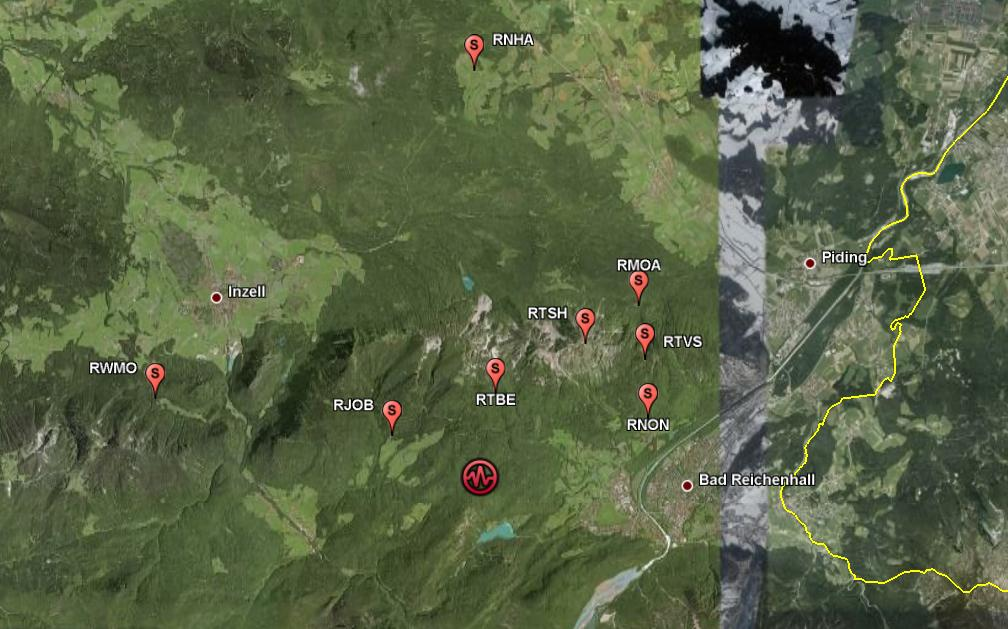
\includegraphics[width=0.8\textwidth]{rh.jpg}
\\[-1ex]{\tiny [http://earth.google.com]}
\end{center}

\exercise{Calculate the Local Magnitude}\\
Use the file \verb#RJOB_WA_CUT.MSEED# to read \verb#MiniSEED# waveform data
from the earthquake. These data have already been simulated to displacement on
a Wood-Anderson seismometer and trimmed to the right time span. Estimate the
peak-to-peak amplitude $amp_{pp}$ as the mean of the maximum minus minimum
amplitude on North and East components in the given short time window. Estimate
the local magnitude $M_l$ using a hypocentral distance of $d_{hypo}=7.1$ (km)
given the formula:
\[
M_l = \log_{10}(\frac{amp_{pp}}{2*1000}) + \log_{10}(\frac{d_{hypo}}{100}) + 0.00301 * (d_{hypo} - 100) + 3
\]
\vspace*{3.0em}

\exercise{Simulate the Wood-Anderson Seismometer}\\
Use the file \verb#RJOB.MSEED# to read the original \verb#MiniSEED# waveform
data. Set up two dictionaries containing the response information of both the
original instrument (an \verb#STS-2#) and the Wood-Anderson seismometer in
poles-and-zeros formulation. Each \verb#paz# dictionary needs to contain
\verb#sensitivity# (overall sensitivity), \verb#gain# (normalization factor),
\verb#poles# and \verb#zeros#. After the instrument simulation, trim the
waveform to a short time window around the origin time
(\verb#2008-04-17T16:00:32Z#) and calculate $M_l$ like in exc. 1. Use the
following values (can be found in the Python file XXX):
{\footnotesize
\begin{verbatim}
    STS-2: 'sensitivity': 2516778600.0
           'gain': 60077000.0
           'poles': [-0.037004+0.037016j, -0.037004-0.037016j, -251.33+0j,
                     -131.04-467.29j, -131.04+467.29j]
           'zeros': [0j, 0j]
    Wood-Anderson: 'sensitivity': 1
                   'gain': 2800
                   'poles': [-6.2832-4.7124j, -6.2832+4.7124j]
                   'zeros': [0j]
\end{verbatim}
}
\vspace*{3.0em}

\exercise{Compare to EMSC Catalog}\\
Fetch a list of events from NERIES/EMSC for the time of the earthquake in the
Hochstaufen region (47.75 N, 12.85 E) using \verb#obspy.neries#. Check the magnitude information in the
catalog.
\vspace*{3.0em}

\exercise{Fetch Data from WebDC}\\
Modify exc. 2 to fetch the data via ArcLink from WebDC using
\verb#obspy.arclink#. Use option \verb#getPAZ=True# to fetch response
information along with the waveform. During instrument simulation use option
\verb#paz_remove='self'# to use the attached \verb#paz# information fetched
from WebDC. Calculate $M_l$ like in exc. 2.
\vspace*{3.0em}

\exercise{Compute Hypocentral Distance}\\
Modify exc. 4 to fetch coordinate information for station \verb#RJOB# along
with the waveform. Use exc. 3 to fetch the event information from NERIES/EMSC.
Use the origin time (stored as \verb#datetime# in the event dictionary) during
the data request instead of the previously hardcoded value. Also calculate the
hypocentral distance dynamically. Use function \verb#utlGeoKm# from module
\verb#obspy.signal# to compute horizontal distances from geographic
coordinates. Calculate $M_l$ like in exc. 4 using the computed hypocentral
distance.
\vspace*{3.0em}

\exercise{Determine Event Onset Using a Triggering Algorithm}\\
Read waveform data from file \verb#RJOB.MSEED# and run a recursive STA/LTA
trigger on the Z component of the data. Compute the approximate event onset
time from \verb#starttime# and \verb#sampling_rate# of the traces and from the
position of the maximum in the triggered data. Store this time in an
\verb#UTCDateTime# object.
\vspace*{3.0em}

\exercise{Use Trigger Time in Magnitude Estimation}\\
Modify exc. 5 to use a dynamically determined trigger time like in exc. 6 for
trimming operations on the data. Calculate $M_l$ like in exc. 5.
\vspace*{3.0em}

\exercise{Estimate Magnitudes for a List of Stations}\\
Modify exc. 7 and use a list of stations (e.g. \verb#RJOB#, \verb#RMOA# and
\verb#RNON#). Loop over this list and estimate the magnitude for each station
individually. (The event onset time and hypocentral distance should be computed
dynamically like in exc. 7.)
\vspace*{3.0em}

\exercise{Fetch List of Available Stations from WebDC}\\
Fetch a list of available stations in network \verb#BW# (BayernNetz) for the
time around the earthquake (\verb#2008-04-17T16:00:32Z#) via ArcLink from
WebDC. Print the station code for every station in the list.
\vspace*{3.0em}

\exercise{Estimate Magnitudes at All Available Stations}\\
Modify exc. 8 to fetch a list of stations like in exc. 9. Loop over this list,
fetch the data and estimate the magnitude for each of the stations.\\ Note:
There is a bug in the station request via arclink such that not all stations in
the response really have data available, you can put the \verb#getWaveform()#
call inside a \verb#try/except# statement like this:
{\footnotesize
\begin{verbatim}
            try:
                client.getWaveform(..., station=sta, ...)
            except:
                print "problem with station:", sta
                continue
\end{verbatim}
}
\vspace*{3.0em}

\exercise{Try Program with Events in Vogtland Swarm Region}\\
By now, the program is rather flexible. We can now change to a completely
different set of events. Modify exc. 10 and change the event request from EMSC
to use events in the Vogtland swarm area (roughly 50.2 N, 12.2 E) at the
north-eastern Bavarian border. There are two magnitude 4+ events in EMSC in
2008 that we can use, for example. Either use one single event like before or
add an additional for loop going through all requested events.
\vspace*{3.0em}

\exercise{Organize Magnitude Estimation in New Python Module}\\
At the end we can clean up the program we wrote by extracting the magnitude
estimation steps in a separate, new Python module. Make a new Python file
\verb#mess_exercise_12_module.py# with a function called
\verb#estimate_magnitude(...)#. This function should take four arguments:
\begin{inparaenum}[\itshape a\upshape)] \item a \verb#Stream# object with Z, N
and E traces with attached paz and coordinate information, \item the longitude
of the event, \item the latitude of the event and \item the depth of the event.
\end{inparaenum} Move and adjust the signal processing steps to this new module
and modify exc. 11 to import and use the function
\verb#estimate_magnitude(...)#.
\vspace*{3.0em}

\end{document}
